\documentclass[11pt]{article}
\usepackage{geometry}                % See geometry.pdf to learn the layout options. There are lots.
\geometry{letterpaper}                   % ... or a4paper or a5paper or ... 
%\geometry{landscape}                % Activate for for rotated page geometry
\usepackage[parfill]{parskip}    % Activate to begin paragraphs with an empty line rather than an indent
\usepackage{daves,fancyhdr,natbib,graphicx,dcolumn,amsmath,lastpage,url}
\usepackage{amsmath,amssymb,epstopdf,longtable}
\usepackage{paralist}  % need to properly formulate standard answer blocks
\usepackage[final]{pdfpages}
\DeclareGraphicsRule{.tif}{png}{.png}{`convert #1 `dirname #1`/`basename #1 .tif`.png}
\pagestyle{fancy}
\lhead{CE 3372 Water Systems Design; Exam 2}
\rhead{Name:\_\_\_\_\_\_\_\_\_\_\_\_\_\_\_\_\_\_\_\_\_\_\_\_\_\_\_\_\_\_\_\_\_\_(1 pts.)}
\lfoot{REVISION A \small{.}}
\cfoot{}
\rfoot{Page \thepage\ of \pageref{LastPage}}
\renewcommand\headrulewidth{0pt}
\newcommand\tab[1][1cm]{\hspace*{#1}}



\begin{document}
%%%%%%%%%%%%%%%%%%%%%%%%%%%%%%%%%%%
\begingroup
\begin{center}
{\textbf{{ CE 3372 Water Systems Design}  \\ Fall 2017} \footnote{For partial credit show work}
}
\end{center}
\endgroup

%%%%%%%%%%%%%%%%%%%%%%%%%%%

\begin{enumerate}
%%%%%%%%%%%%%%%%%%%%%%%%%%%%%%%%%%%%%%%%%%%%%%
%%%%%%%% PROBLEM 1 %%%%%%%%%%%%%%%%%%%%%%%%%%%%%%%
%%%%%%%%%%%%%%%%%%%%%%%%%%%%%%%%%%%%%%%%%%%%%%
\item  (1 pts.)
The hydraulic radius in a conduit containing a flowing liquid is
\begin{enumerate} [(A)]
\item	the ratio of the cross-sectional area of flow and the wetted perimeter
\item	the mean radius from the center of flow to the wetted side of the conduit
\item	the ratio of the cross-sectional area of the conduit and the wetted perimeter
\item	the ratio of the wetted perimeter and the cross-sectional area of the conduit
\end{enumerate}
%%%%%%%%%%%%%%%%%%%%%%%%%%%%%%%%%%%%%%%%%%%%%%
%%%%%%%% PROBLEM 2 %%%%%%%%%%%%%%%%%%%%%%%%%%%%%%%
%%%%%%%%%%%%%%%%%%%%%%%%%%%%%%%%%%%%%%%%%%%%%%
\item (5 pts.)
The rational runoff coefficient for a $14.81$~acre parcel property is $0.35$.  
The rainfall intensity is $4.56$ inches per hour.  
The peak discharge from this property is anticipated to be about
%standard answer set
\begin{enumerate} [(A)]
\item $23.82$ cfs
\item $33.01$ cfs
\item $48.18$ cfs
\item $57.86$ cfs
\item $65.90$ cfs
\item $80.18$ cfs
\item $97.81$ cfs
\end{enumerate}
%%%%%%%%%%%%%%%%%%%%%%%%%%%%%%%
% C=0.35, i = 4.56, A = 14.81, Qp=   23.82 % %
% C=0.85, i = 4.56, A = 14.81, Qp=   57.86 % %
% C=0.35, i = 6.54, A = 14.31, Qp=   33.01 % %
% C=0.85, i = 6.54, A = 14.31, Qp=   80.18% %
%%%%%%%%%%%%%%%%%%%%%%%%%%%%%%%
\item  (8 pts.)
A storm sewer (reinforced concrete pipe) is 400-feet long and 36-inches in diameter.  The sewer flows from a junction box (invert elevation $101.00$ feet) to a lift station sump (invert elevation $100.00$ feet).  Assuming Manning's roughness coefficient is $0.013$ for all flow depths, the full-sewer flow is about% US Customary Versions
\begin{enumerate} [(A)]
\item  $17.8$ cfs
\item  $19.2$ cfs
\item  $22.1$ cfs
\item  $28.9$ cfs
\item  $31.2$ cfs
\item  $33.4$ cfs
\item  $35.9$ cfs
\item  $36.4$ cfs
\end{enumerate}
%%%%%%%%%%%%%%%%%%%%%%%%%%%%%%%
% n=0.013, So = 1/400, D = 30/12, Qf = 20.6 , Q= 22.1    % %
% n=0.013, So = 1/400, D = 36/12, Qf = 33.4 , Q = 35.9    % %
% n=0.015, So = 1/400, D = 30/12, Qf = 17.8 , Q= 19.1     %%
% n=0.015, So = 1/400, D = 36/12, Qf = 28.9 , Q = 31.2    %%
%%%%%%%%%%%%%%%%%%%%%%%%%%%%%%%


%%%%%%%%%%%%%%%%%%%%%%%%%%%%%%%%%%%%%%%%%%%%%%
%%%%%%%% PROBLEM 3 BEGIN %%%%%%%%%%%%%%%%%%%%%%%%%%%
%%%%%%%%%%%%%%%%%%%%%%%%%%%%%%%%%%%%%%%%%%%%%%
%====== SOLUTION ==========================
% C  use Manning's equation for full pipe flow
%  NCEES pp 160-161
%==========================================
%=======================================================================
\clearpage
\item (8 pts.)
The storm sewer in the question above is flowing at $\frac{3}{4}$ full.  What is the discharge in the sewer?
%standard answer set
\begin{enumerate} [(A)]
\item  $Q_{75\%}= 16.9$ cfs
\item  $Q_{75\%}= 18.2$ cfs
\item  $Q_{75\%}= 20.1$ cfs
\item  $Q_{75\%}= 27.5$ cfs
\item  $Q_{75\%}= 32.3$ cfs
\item  $Q_{75\%}= 31.7$ cfs
\item  $Q_{75\%}= 34.1$ cfs
\item  $Q_{75\%}= 34.5$ cfs
\end{enumerate}
%%%%%%%%%%%%%%%%%%%%%%%%%%%%%%%%%%%%%%%%%%%%%%
%%%%%%%% PROBLEM 4 DONE %%%%%%%%%%%%%%%%%%%%%%%%%%%
%%%%%%%%%%%%%%%%%%%%%%%%%%%%%%%%%%%%%%%%%%%%%%


%%%%%%%%%%%%%%%%%%%%%%%%%%%%%%%%%%%%%%%%%%%%%%
%%%%%%%% PROBLEM 5 %%%%%%%%%%%%%%%%%%%%%%%%%%%
%%%%%%%%%%%%%%%%%%%%%%%%%%%%%%%%%%%%%%%%%%%%%%
\clearpage
\item (8 pts.)\label{prob:VChannel}
A triangular V-shaped channel is depicted in Figure \ref{fig:TriangleChannel}.  
The channel's dimensionless slope in the direction of flow is $0.008$. 
Manning's $N$ for the channel is $n = 0.012$.  
The flow width at the surface is $T = 2$ meters.\footnote{Show your work on the next page for full credit.}
\begin{figure}[h!] %  figure placement: here, top, bottom, or page
\centering
   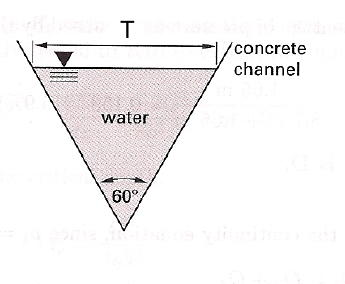
\includegraphics[width=2.2in]{TriangleChannel.jpg}
   \caption{Triangular channel.}
   \label{fig:TriangleChannel} 
\end{figure}
\begin{enumerate}[A)]
\item What is the flow width? \\~\\
\begin{tabular}{p{2in} p{2in}  } 
(A) $1$~m & (E) $5$~m \\ 
(B) $2$~m & (F) $6$~m  \\
(C) $3$~m & (G) $7$~m  \\
(D) $4$~m & (H) $8$~m  \\
\end{tabular}
\item What is the flow depth?\\~\\
\begin{tabular}{p{2in} p{2in}  } 
(A) $1$~m & (E) $5$~m \\ 
(B) $2$~m & (F) $6$~m  \\
(C) $3$~m & (G) $7$~m  \\
(D) $4$~m & (H) $8$~m  \\
\end{tabular}
\item What is the wetted perimeter?\\~\\
\begin{tabular}{p{2in} p{2in}  } 
(A) $2$~m & (E) $10$~m \\ 
(B) $4$~m & (F) $12$~m  \\
(C) $6$~m & (G) $14$~m  \\
(D) $8$~m & (H) $16$~m  \\
\end{tabular}

\item What is the flow area?\\~\\
\begin{tabular}{p{2in} p{2in}  } 
A) $111$~m$^3$/s & E) $111$~m$^3$/s \\ 
B) $111$~m$^3$/s & F) $111$~m$^3$/s  \\
C) $111$~m$^3$/s & G) $111$~m$^3$/s  \\
D) $111$~m$^3$/s & H) $111$~m$^3$/s  \\
\end{tabular}

\item What is the flow rate using Manning's equation?\\~\\
\begin{tabular}{p{2in} p{2in}  } 
A) $111$~m$^3$/s & E) $111$~m$^3$/s \\ 
B) $111$~m$^3$/s & F) $111$~m$^3$/s  \\
C) $111$~m$^3$/s & G) $111$~m$^3$/s  \\
D) $111$~m$^3$/s & H) $111$~m$^3$/s  \\
\end{tabular}

\end{enumerate}

Show work for Problem \ref{prob:VChannel} below:
\clearpage
\item  (11 pts.) \label{prob:CircularSewer}
A partially-full pipe with a radius of $r$ meters is depicted in Figure \ref{fig:CircularSewer}.
The angle shown is $\alpha~=~ 70^o$

\begin{figure}[h!] %  figure placement: here, top, bottom, or page
\centering
   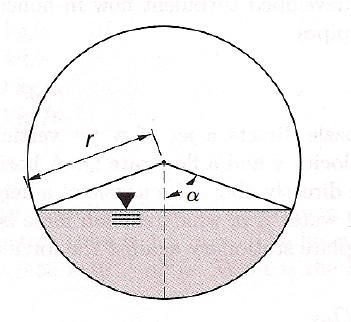
\includegraphics[width=1.9in]{CircularSewer.jpg}
   \caption{Circular channel flowing partially full.}
   \label{fig:CircularSewer} 
\end{figure}

\begin{enumerate}[A)]
\item What is the angle in radians? \\~\\
\begin{tabular}{p{2in} p{2in}  } 
(A) $1$~m & (E) $5$~m \\ 
(B) $2$~m & (F) $6$~m  \\
(C) $3$~m & (G) $7$~m  \\
(D) $4$~m & (H) $8$~m  \\
\end{tabular}
\item What is the flow depth?\\~\\
\begin{tabular}{p{2in} p{2in}  } 
(A) $1$~m & (E) $5$~m \\ 
(B) $2$~m & (F) $6$~m  \\
(C) $3$~m & (G) $7$~m  \\
(D) $4$~m & (H) $8$~m  \\
\end{tabular}
\item What is the wetted perimeter?\\~\\
\begin{tabular}{p{2in} p{2in}  } 
(A) $2$~m & (E) $10$~m \\ 
(B) $4$~m & (F) $12$~m  \\
(C) $6$~m & (G) $14$~m  \\
(D) $8$~m & (H) $16$~m  \\
\end{tabular}
\item What is the hydraulic radius?\\~\\
\begin{tabular}{p{2in} p{2in}  } 
(A) $2$~m & (E) $10$~m \\ 
(B) $4$~m & (F) $12$~m  \\
(C) $6$~m & (G) $14$~m  \\
(D) $8$~m & (H) $16$~m  \\
\end{tabular}

\item What is the flow area?\\~\\
\begin{tabular}{p{2in} p{2in}  } 
A) $111$~m$^3$/s & E) $111$~m$^3$/s \\ 
B) $111$~m$^3$/s & F) $111$~m$^3$/s  \\
C) $111$~m$^3$/s & G) $111$~m$^3$/s  \\
D) $111$~m$^3$/s & H) $111$~m$^3$/s  \\
\end{tabular}

\item What is the flow rate using Manning's equation?\\~\\
\begin{tabular}{p{2in} p{2in}  } 
A) $111$~m$^3$/s & E) $111$~m$^3$/s \\ 
B) $111$~m$^3$/s & F) $111$~m$^3$/s  \\
C) $111$~m$^3$/s & G) $111$~m$^3$/s  \\
D) $111$~m$^3$/s & H) $111$~m$^3$/s  \\
\end{tabular}

\end{enumerate}


What is the hydraulic radius of flow in the circular section?
%standard answer set
\begin{enumerate} [(A)]
\item $0.44$ m
\item $0.88$ m
\item $1.30$ m
\item $1.80$ m
\item $0.44$ m
\item $0.88$ m
\item $1.30$ m
\item $1.80$ m
\end{enumerate}

Show work for Problem \ref{prob:CircularSewer} below:

%\item $0.24$~cms (cubic meters per second)
%\item $0.31$~cms 
%\item $3.52$~cms 
%\item $3.91$~cms 
%\item $4.41$~cms 
%\item $4.45$~cms 
%\item $5.57$~cms 
%\item $6.66$~cms 
%\item $7.38$~cms 
%\item $9.31$~cms 

%%%%%%%%%%%%%%%%%%%%%%%%%%%%%%%
% n=0.012, So = 0.005, Q= 4.41 m/s % %
% n=0.015, So = 0.005, Q=  3.52 m/s % %
% n=0.012, So = 0.008, Q=   5.57 m/s %%
% n=0.015, So = 0.008, Q=   4.45 m/s %%
%%%%%%%%%%%%%%%%%%%%%%%%%%%%%%%%

%%%%%%%%%%%%%%%%%%%%%%%%%%%%%%%%%%%%%%%%%%%%%%%
%%%%%%%% EPA PROBLEM BEGIN %%%%%%%%%%%%%%%%%%%%%%%%%%%
%%%%%%%%%%%%%%%%%%%%%%%%%%%%%%%%%%%%%%%%%%%%%%%

\clearpage
\item (46 pts.)
 An EPA-NET simulation model for a reservoir-pump-network was constructed and operated for four (4) different operational scenarios.   Figure \ref{fig:epa-net-map-gpm} is a depiction of the network.   The numbers next to the nodes are Node\_ID values in the reports that follow, and the numbers next to the pipes are the Link\_ID values.  The network is supplied from a reservoir through a booster pump, both are depicted on Figure \ref{fig:epa-net-map-gpm}. 

\begin{figure}[h!] %  figure placement: here, top, bottom, or page
\centering
   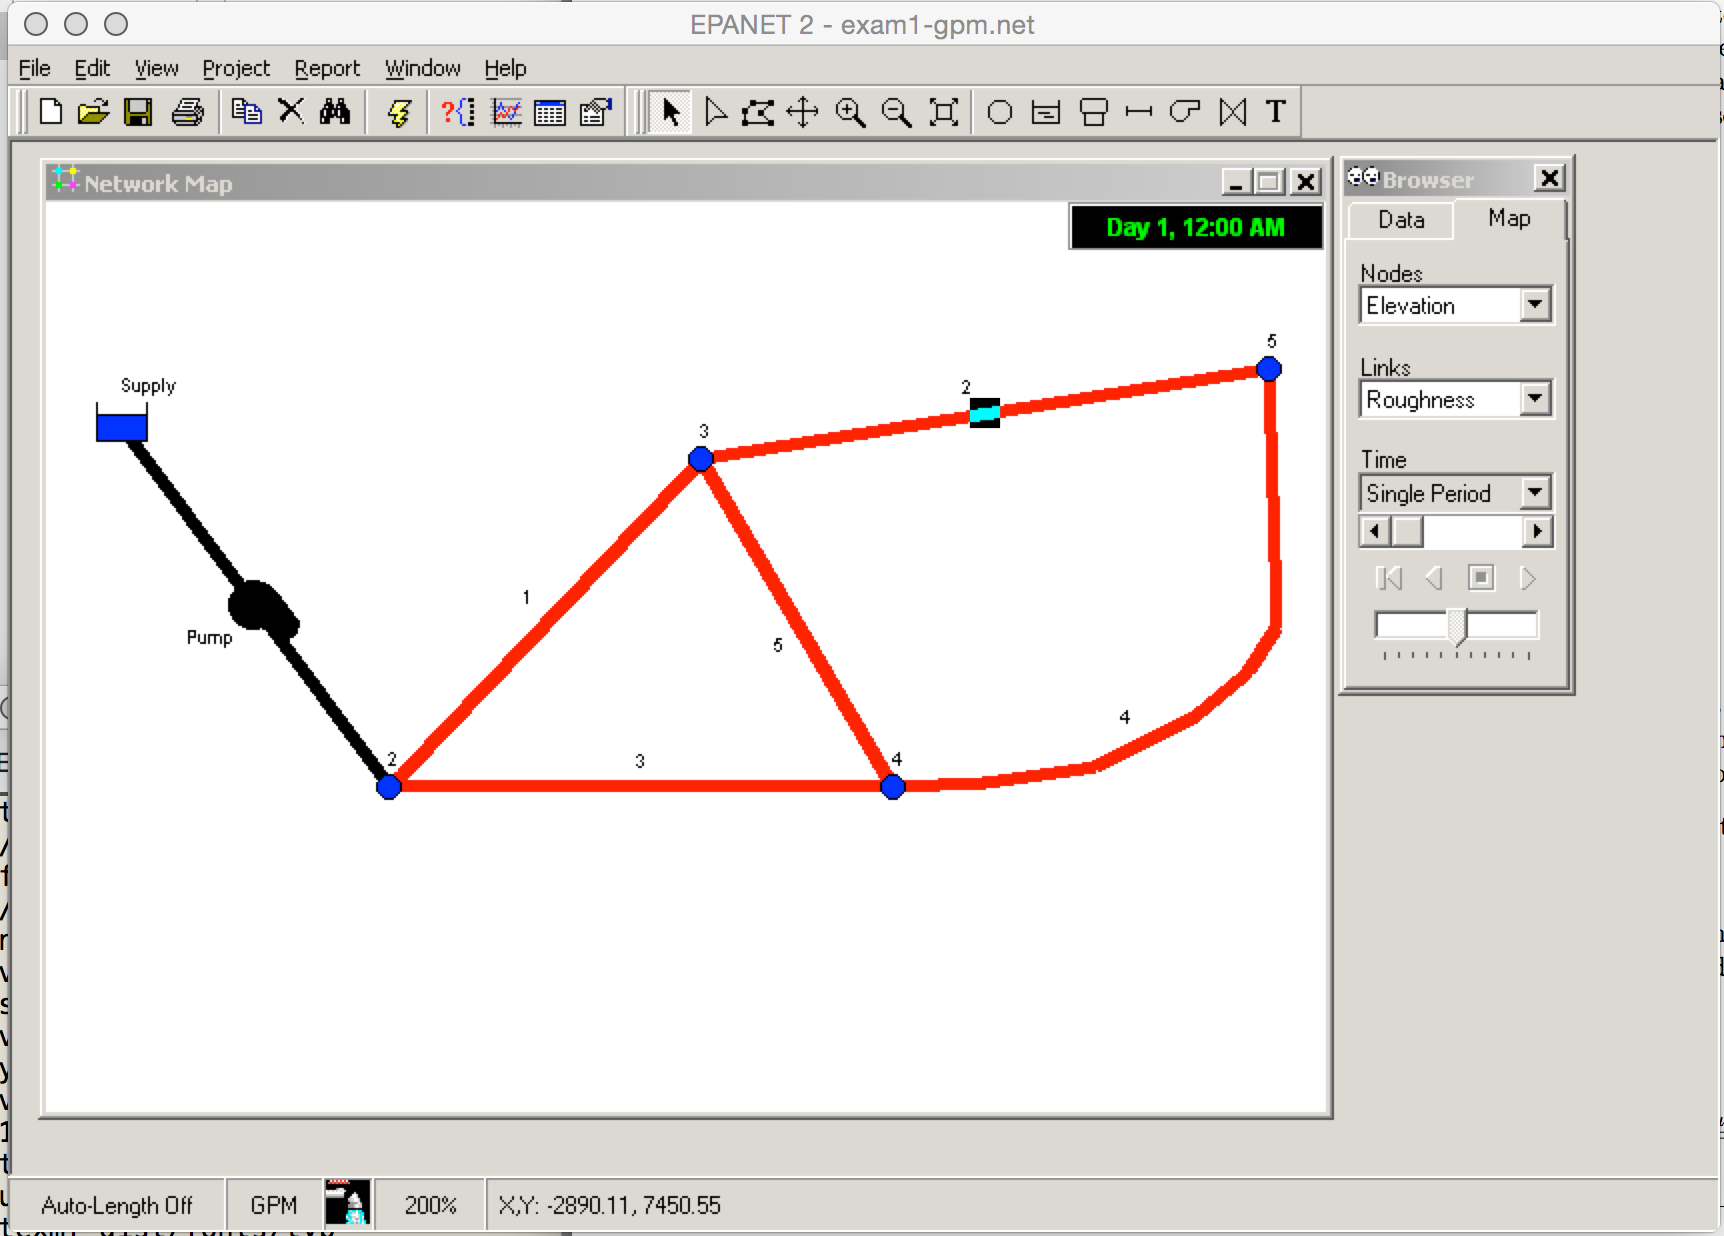
\includegraphics[width=6in]{epa-net-map-gpm.jpg}
   \caption{EPA-NET system topology.}
   \label{fig:epa-net-map-gpm} 
\end{figure}

Figure \ref{fig:epanet1} is an output report for simulation 1.   \\
Figure \ref{fig:epanet2} is an output report for simulation 2. \\  
Figure \ref{fig:epanet3} is an output report for simulation 3.  \\
Figure \ref{fig:epanet4} is an output report for simulation 4.  \\

These four simulation represent different demand scenarios for the same system.  
Interpret these reports, to answer the following questions:
\newpage
\begin{enumerate}[a)]
\item Which of the four simulations most closely represents a shut-off (zero discharge) condition?
\begin{enumerate}[A)]
\item Simulation \#1.
\item Simulation \#2.
\item Simulation \#3.
\item Simulation \#4.
\end{enumerate}

\item What is the total head at the supply reservoir for each simulation?
\begin{enumerate}[A)]
\item $\approx$~0 ft.
%\item $\approx$~0 m.
\item $\approx$~31 ft.
%\item $\approx$~31 m.
\item $\approx$~100 ft.
\item $\approx$~100 m. 
%\item A and B.
%\item C and D.
%\item D and E.
%\item E and F.
%\item all of the above.
%\item none of the above.
\end{enumerate}

\item What is the total head at node \#2 for simulation \#1?
\begin{enumerate}[A)]
\item $\approx$~113 ft.
\item $\approx$~117 ft.
\item $\approx$~118 ft.
\item $\approx$~120 ft. 
%\item A and B.
%\item C and D.
%\item D and E.
%\item E and F.
%\item all of the above.
%\item none of the above.
\end{enumerate}

\item What is the total head at node \#2 for simulation \#2?
\begin{enumerate}[A)]
\item $\approx$~113 ft.
\item $\approx$~117 ft.
\item $\approx$~118 ft.
\item $\approx$~120 ft. 
%\item A and B.
%\item C and D.
%\item D and E.
%\item E and F.
%\item all of the above.
%\item none of the above.
\end{enumerate}

\item What is the total head at node \#2 for simulation \#3?
\begin{enumerate}[A)]
\item $\approx$~113 ft.
\item $\approx$~117 ft.
\item $\approx$~118 ft.
\item $\approx$~120 ft. 
%\item A and B.
%\item C and D.
%\item D and E.
%\item E and F.
%\item all of the above.
%\item none of the above.
\end{enumerate}
\newpage

\item What is the total head at node \#2 for simulation \#4?
\begin{enumerate}[A)]
\item $\approx$~113 ft.
\item $\approx$~117 ft.
\item $\approx$~118 ft.
\item $\approx$~120 ft. 
%\item A and B.
%\item C and D.
%\item D and E.
%\item E and F.
%\item all of the above.
%\item none of the above.
\end{enumerate}


\item Complete the table below.  $Q_{pump}$ is the discharge in gallons-per-minute through the pump station, $H_{Supply}$ is the head at the supply reservoir,  $H_{Node2}$ is the head at Node 2, and $\Delta H_{pump} =  H_{Node2} - H_{Supply}$ is the added head supplied by the pump.
% Requires the booktabs if the memoir class is not being used
\begin{table}[htbp]
   \centering
      \caption{Pump Discharge and Supplied Head}
   \begin{tabular}{p{1in} p{1in} p{1in} p{1in} p{1in} } % Column formatting, @{} suppresses leading/trailing space
Simulation \# & $Q_{pump}$ & $H_{Supply}$ & $H_{Node2}$ & $\Delta H_{pump}$ \\
\hline
\hline
~~1 & ~ &~ & ~ & ~ \\
~ & ~ &~ & ~ & ~ \\
\hline
~~2 & ~ &~ & ~ & ~ \\
~ & ~ &~ & ~ & ~ \\
\hline
~~3 & ~ &~ & ~ & ~\\
~ & ~ &~ & ~ & ~ \\
\hline
~~4 & ~ &~ & ~ & ~ \\
~ & ~ &~ & ~ & ~ \\
\hline
   \end{tabular}
   \label{tab:pump-curve}
\end{table}

\item Complete the table below.  $Q_{pump}$ is the discharge in gallons-per-minute through the pump station, $\Delta H_{Node 2 -to- 5}$ is head loss in the system from Node 2 to Node 5.
\begin{table}[htbp]
   \centering
      \caption{System Discharge and Head Loss}
   \begin{tabular}{p{1in} p{1in} p{1in} p{1in} p{1in} } % Column formatting, @{} suppresses leading/trailing space
Simulation \# & $Q_{pump}$ & $H_{Node2}$ & $H_{Node5}$ & $\Delta H_{Node 2 -to- 5}$ \\
\hline
\hline
~~1 & ~ &~ & ~ & ~ \\
~ & ~ &~ & ~ & ~ \\
\hline
~~2 & ~ &~ & ~ & ~ \\
~ & ~ &~ & ~ & ~ \\
\hline
~~3 & ~ &~ & ~ & ~\\
~ & ~ &~ & ~ & ~ \\
\hline
~~4 & ~ &~ & ~ & ~ \\
~ & ~ &~ & ~ & ~ \\
\hline
   \end{tabular}
   \label{tab:system-curve}
\end{table}
\newpage

\item Sketch and the pump curve on Figure \ref{fig:BlankPumpCurve} below. 

\begin{figure}[h!] %  figure placement: here, top, bottom, or page
\centering
   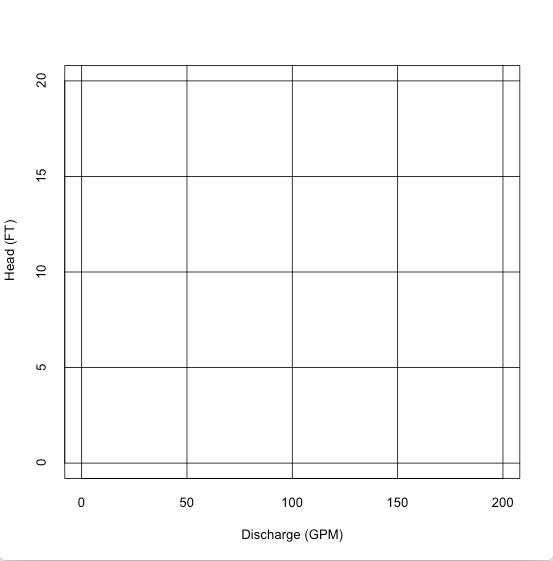
\includegraphics[width=6in]{BlankPumpCurve.jpg}
   \caption{Pump Performance Curve}
   \label{fig:BlankPumpCurve} 
\end{figure}
\clearpage
\item Estimate the value of $K_{system}$ if the pump performance curve has the mathematical structure: 
$\Delta H_{pump} = H_{shutoff} - K_{system} \times Q_{pump}^2$, 
\\
\\
\\
\\
\\
\\
\\
\\
\\
\\
\\
\\
\\
\\
\\
\\
\\
\\
\\
\\

\item Estimate the value of $K_{loss}$ if the system loss curve has the mathematical structure:
 $\Delta H_{Node~2 -to- 5}~= K_{loss} \times Q_{pump}^2$, 
\\
\\
\\
\\
\\
\\
\\
\\
\\
\\
\\
\\
\\
\\
\\
\\
\\
\\
\\
\\



\item Estimate the discharges, head losses, and nodal heads if pipes 4 and 5 are removed and the nodal demands are as shown on Figure \ref{fig:epa-net-map-gpm-no5}. (Same demand as Simulation \# 2.)\footnote{Most, but not all, answers appear in the simulation reports -- you will have to interpolate one head loss value from different simulation reports to complete the problem.}
\begin{figure}[h!] %  figure placement: here, top, bottom, or page
\centering
   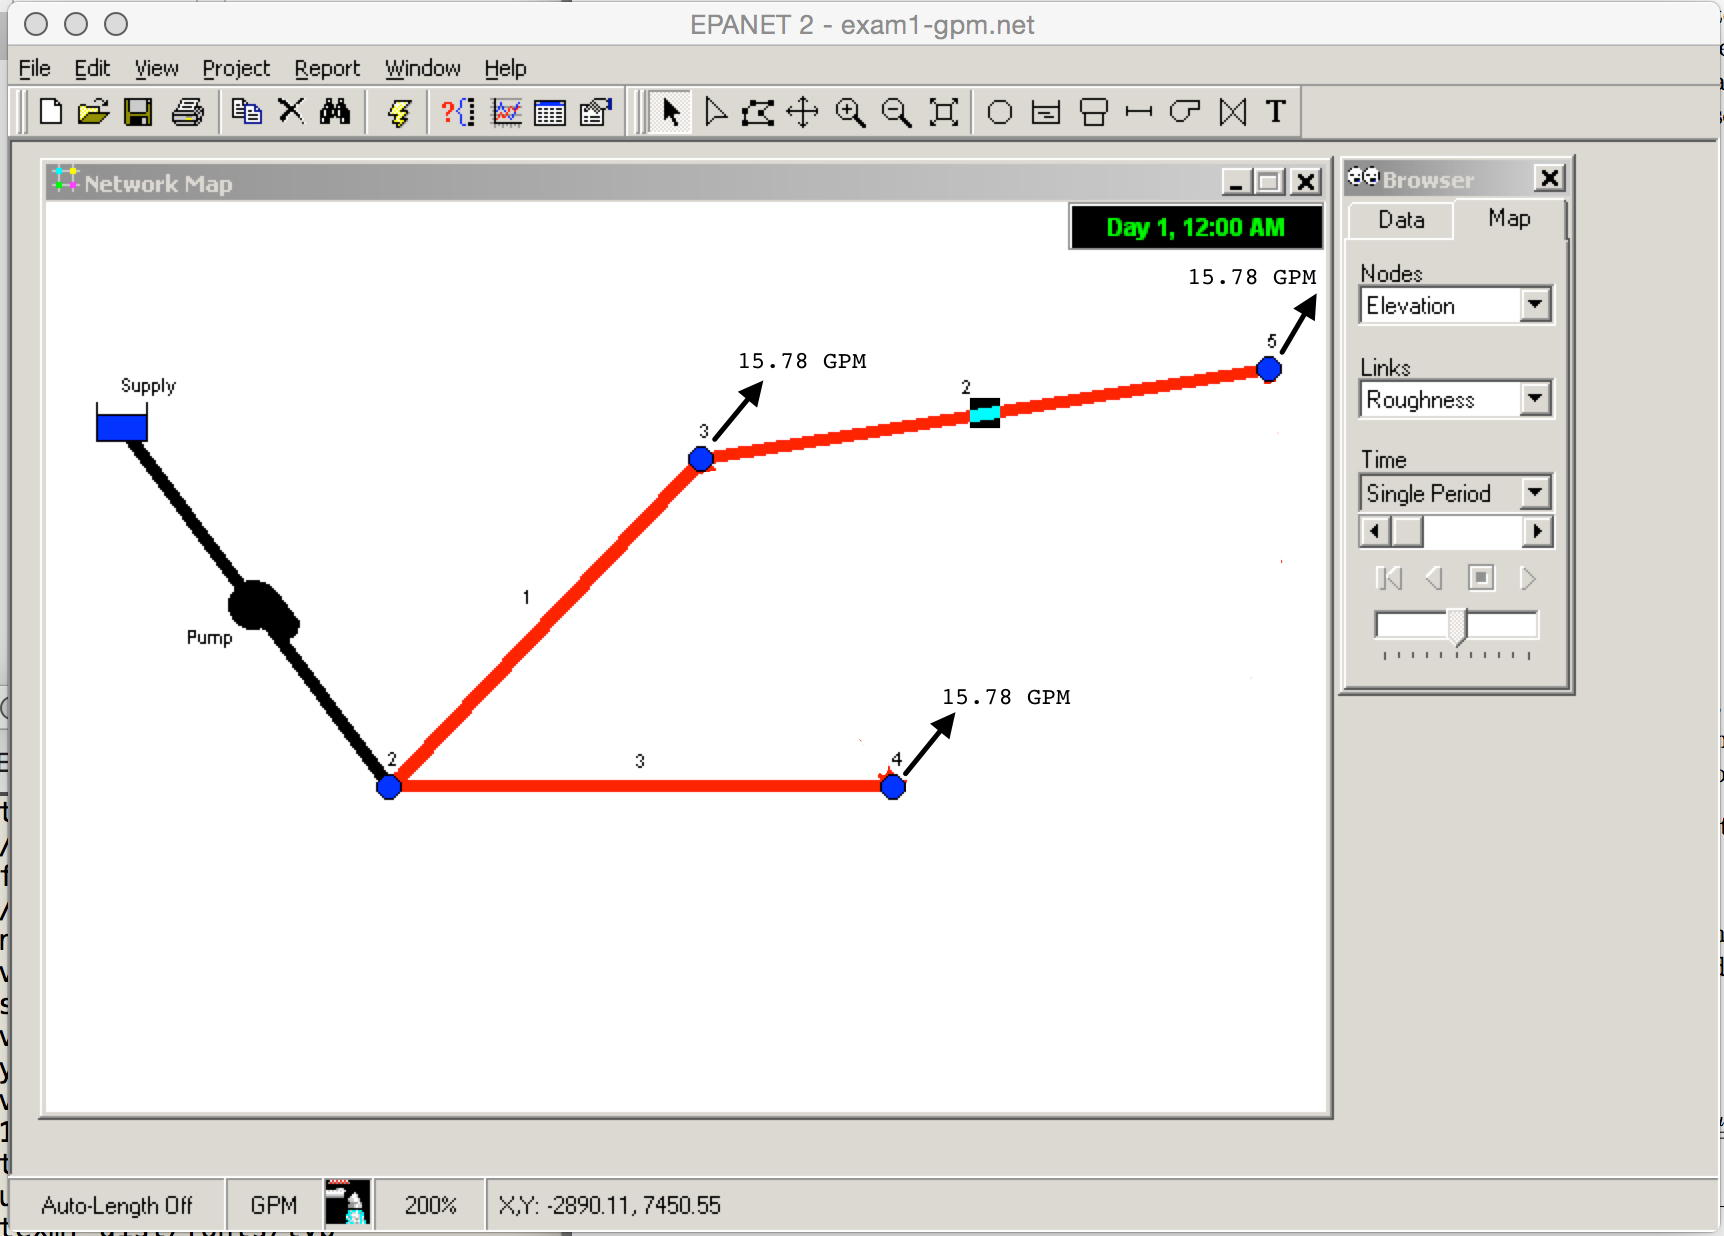
\includegraphics[width=6in]{epa-net-map-gpm-no5.jpg}
   \caption{EPA-NET system topology.}
   \label{fig:epa-net-map-gpm-no5} 
\end{figure}

\begin{enumerate}[A)]
\item Pipe \#1 Discharge = \_\_\_\_\_\_\_\_\_\_\_\_\_\_\_~ GPM.\\~\\
\item Pipe \#2 Discharge = \_\_\_\_\_\_\_\_\_\_\_\_\_\_\_~ GPM.\\~\\
\item Pipe \#3 Discharge = \_\_\_\_\_\_\_\_\_\_\_\_\_\_\_~ GPM.\\~\\
\newpage ~\\~\\
\item Pipe \#1 Head Loss = \_\_\_\_\_\_\_\_\_\_\_\_\_\_\_~ FT.\\~\\~\\
\item Pipe \#2 Head Loss = \_\_\_\_\_\_\_\_\_\_\_\_\_\_\_~ FT.\\~\\~\\
\item Pipe \#3 Head Loss = \_\_\_\_\_\_\_\_\_\_\_\_\_\_\_~ FT. \\~\\~\\
\item Node \#2 Head = \_\_\_\_\_\_\_\_\_\_\_\_\_\_\_~ FT.\\~\\~\\
\item Node \#3 Head = \_\_\_\_\_\_\_\_\_\_\_\_\_\_\_~ FT.\\~\\~\\
\item Node \#5 Head = \_\_\_\_\_\_\_\_\_\_\_\_\_\_\_~ FT.\\~\\~\\
\end{enumerate}
\end{enumerate} 


%%% YOUR ON YOUR OWN %%%%%%%%%%%%%%%%%%%%
\begin{figure}[ht!] %  figure placement: here, top, bottom, or page
\centering
\begin{verbatim}
  Page 1                                    Thu Mar 23 15:44:27 2017

  ******************************************************************
  *                           E P A N E T                          *
  *                   Hydraulic and Water Quality                  *
  *                   Analysis for Pipe Networks                   *
  *                         Version 2.00.12                        *
  ******************************************************************
  
  Analysis begun Thu Mar 23 15:44:27 2017

   
  Hydraulic Status:
  -----------------------------------------------------------------------
     0:00:00: Balanced after 7 trials
     0:00:00: Reservoir 1 is closed
   
   
  Node Results:
  --------------------------------------------------------
                  Elevation    Demand      Head  Pressure
  Node                   ft       gpm        ft       psi
  --------------------------------------------------------
  2                  100.00      0.00    120.00      8.67
  3                  100.00      0.01    120.00      8.67
  4                  100.00      0.01    120.00      8.67
  5                  100.00      0.01    120.00      8.67
  1                  100.00     -0.03    100.00      0.00  Reservoir
   
   
  Link Results:
  ----------------------------------------------------------------------------
                     Length  Diameter      Flow  Velocity  Headloss  F-Factor
  Link                   ft        in       gpm       fps   /1000ft          
  ----------------------------------------------------------------------------
  1                 3280.00      5.00      0.07      0.00      0.00     0.279
  2                 3280.00      5.00     -0.05      0.00      0.00     0.271
  3                 3280.00      5.00     -0.04      0.00      0.00     0.840
  4                 3280.00      5.00      0.06      0.00      0.00     0.189
  5                 1000.00      5.00      0.11      0.00      0.00     0.000
  6                    0.00     12.00      0.03      0.00    -20.00     0.000  Pump
   
  Analysis ended Thu Mar 23 15:44:27 2017
  \end{verbatim}
     \caption{EPA-NET Report, Simulation \#1}
   \label{fig:epanet1} 
\end{figure}
%%%%%%%%%%%%%%%%%%%%%%%%%%%%%%%%%%%%%%
%%%%%%%%%%%%%%%%%%%%%%%%%%%%%%%%%%%%%%

\begin{figure}[ht!] %  figure placement: here, top, bottom, or page
\centering
\begin{verbatim}
  Page 1                                    Thu Mar 23 15:45:45 2017

  ******************************************************************
  *                           E P A N E T                          *
  *                   Hydraulic and Water Quality                  *
  *                   Analysis for Pipe Networks                   *
  *                         Version 2.00.12                        *
  ******************************************************************
  
  Analysis begun Thu Mar 23 15:45:45 2017

   
  Hydraulic Status:
  -----------------------------------------------------------------------
     0:00:00: Balanced after 5 trials
     0:00:00: Reservoir 1 is emptying
   
   
  Node Results:
  --------------------------------------------------------
                  Elevation    Demand      Head  Pressure
  Node                   ft       gpm        ft       psi
  --------------------------------------------------------
  2                  100.00      0.00    118.74      8.12
  3                  100.00     15.78    118.15      7.86
  4                  100.00     15.78    118.15      7.86
  5                  100.00     15.78    118.06      7.83
  1                  100.00    -47.34    100.00      0.00  Reservoir
   
   
  Link Results:
  ----------------------------------------------------------------------------
                     Length  Diameter      Flow  Velocity  Headloss  F-Factor
  Link                   ft        in       gpm       fps   /1000ft          
  ----------------------------------------------------------------------------
  1                 3280.00      5.00     23.67      0.39      0.18     0.032
  2                 3280.00      5.00      7.89      0.13      0.03     0.041
  3                 3280.00      5.00     23.67      0.39      0.18     0.032
  4                 3280.00      5.00      7.89      0.13      0.03     0.041
  5                 1000.00      5.00      0.00      0.00      0.00   408.583
  6                    0.00     12.00     47.34      0.00    -18.74     0.000  Pump
   
  Analysis ended Thu Mar 23 15:45:45 2017  \end{verbatim}
     \caption{EPA-NET Summary Report, Simulation \#2}
   \label{fig:epanet2} 
\end{figure}
%%%%%%%%%%%%%%%%%%%%%%%%%%%%%%%%%%%%%%%%
%%%%%%%%%%%%%%%%%%%%%%%%%%%%%%%%%%%%%%%%
\begin{figure}[ht!] %  figure placement: here, top, bottom, or page
\centering
\begin{verbatim}
  Page 1                                    Thu Mar 23 15:49:29 2017

  ******************************************************************
  *                           E P A N E T                          *
  *                   Hydraulic and Water Quality                  *
  *                   Analysis for Pipe Networks                   *
  *                         Version 2.00.12                        *
  ******************************************************************
  
  Analysis begun Thu Mar 23 15:49:29 2017

   
  Hydraulic Status:
  -----------------------------------------------------------------------
     0:00:00: Balanced after 5 trials
     0:00:00: Reservoir 1 is emptying
   
   
  Node Results:
  --------------------------------------------------------
                  Elevation    Demand      Head  Pressure
  Node                   ft       gpm        ft       psi
  --------------------------------------------------------
  2                  100.00      0.00    117.12      7.42
  3                  100.00     31.56    114.98      6.49
  4                  100.00     31.56    114.98      6.49
  5                  100.00     31.56    114.69      6.37
  1                  100.00    -94.68    100.00      0.00  Reservoir
   
   
  Link Results:
  ----------------------------------------------------------------------------
                     Length  Diameter      Flow  Velocity  Headloss  F-Factor
  Link                   ft        in       gpm       fps   /1000ft          
  ----------------------------------------------------------------------------
  1                 3280.00      5.00     47.34      0.77      0.65     0.029
  2                 3280.00      5.00     15.78      0.26      0.09     0.035
  3                 3280.00      5.00     47.34      0.77      0.65     0.029
  4                 3280.00      5.00     15.78      0.26      0.09     0.035
  5                 1000.00      5.00      0.00      0.00      0.00   702.884
  6                    0.00     12.00     94.68      0.00    -17.12     0.000  Pump
   
  Analysis ended Thu Mar 23 15:49:29 2017

  \end{verbatim}
     \caption{EPA-NET Summary Report, Simulation \#3}
   \label{fig:epanet3} 
\end{figure}
%%%%%%%%%%%%%%%%%%%%%%%%%%%%%%%%%%%%%%%%%%
%%%%%%%%%%%%%%%%%%%%%%%%%%%%%%%%%%%%%%%%%%
\begin{figure}[ht!] %  figure placement: here, top, bottom, or page
\centering
\begin{verbatim}
  Page 1                                    Thu Mar 23 15:51:16 2017

  ******************************************************************
  *                           E P A N E T                          *
  *                   Hydraulic and Water Quality                  *
  *                   Analysis for Pipe Networks                   *
  *                         Version 2.00.12                        *
  ******************************************************************
  
  Analysis begun Thu Mar 23 15:51:16 2017

   
  Hydraulic Status:
  -----------------------------------------------------------------------
     0:00:00: Balanced after 4 trials
     0:00:00: Reservoir 1 is emptying
   
   
  Node Results:
  --------------------------------------------------------
                  Elevation    Demand      Head  Pressure
  Node                   ft       gpm        ft       psi
  --------------------------------------------------------
  2                  100.00      0.00    113.52      5.86
  3                  100.00     47.34    108.91      3.86
  4                  100.00     47.34    108.91      3.86
  5                  100.00     47.34    108.32      3.60
  1                  100.00   -142.02    100.00      0.00  Reservoir
   
   
  Link Results:
  ----------------------------------------------------------------------------
                     Length  Diameter      Flow  Velocity  Headloss  F-Factor
  Link                   ft        in       gpm       fps   /1000ft          
  ----------------------------------------------------------------------------
  1                 3280.00      5.00     71.01      1.16      1.41     0.028
  2                 3280.00      5.00     23.67      0.39      0.18     0.032
  3                 3280.00      5.00     71.01      1.16      1.41     0.028
  4                 3280.00      5.00     23.67      0.39      0.18     0.032
  5                 1000.00      5.00      0.01      0.00      0.00   180.889
  6                    0.00     12.00    142.02      0.00    -13.52     0.000  Pump
   
  Analysis ended Thu Mar 23 15:51:16 2017  \end{verbatim}
     \caption{EPA-NET Summary Report, Simulation \#4}
   \label{fig:epanet4} 
\end{figure}
\clearpage

\item (30 pts) Figures \ref{fig:waterQ1},\ref{fig:waterQ2}, and \ref{fig:waterQ3} are screen captures of an EPANET extended period simulation for water quality in a pipeline distribution network.
The chemical parameter of interest is Chloramine.  Interpret the figures to answer the following questions: ~\\
\begin{enumerate}[A)]
\item What is the Chloramine value (dosage) in the supply reservoir? \\~\\~\\~\\~\\~\\~\\
\item What is the simulation time, in hours, of the first arrival of chloramine to Node 6? \\~\\~\\~\\~\\~\\~\\
\item What is the distance, in feet, from the supply reservoir to Node 6 along the path that involves Link 11 $->$ Link 1 $->$ Link 4 $->$ Link 7? \\~\\~\\~\\~\\~\\~\\
\item What is the travel time, in hours, along the path above? (Show your calculations) \\~\\~\\~\\~\\~\\~\\
\newpage
\item What is the distance, in feet, from the supply reservoir to Node 6 along the path that involves Link 11 $->$ Link 3 $->$ Link 6 $->$ Link 7? \\~\\~\\~\\~\\~\\~\\
\item What is the travel time, in hours, along the path above? (Show your calculations) \\~\\~\\~\\~\\~\\~\\
\item Are these two times less than 6 hours? \\~\\~\\~\\
\item What is your estimate of the concentration at Node 6 at simulation hour 6:00? \\~\\~\\
\item What is your estimate of the concentration at Node 6 at simulation hour 12:00? \\~\\~\\
\item Explain your reasoning for the two answers above.
\end{enumerate}

\begin{figure}[ht!] %  figure placement: here, top, bottom, or page
\centering
   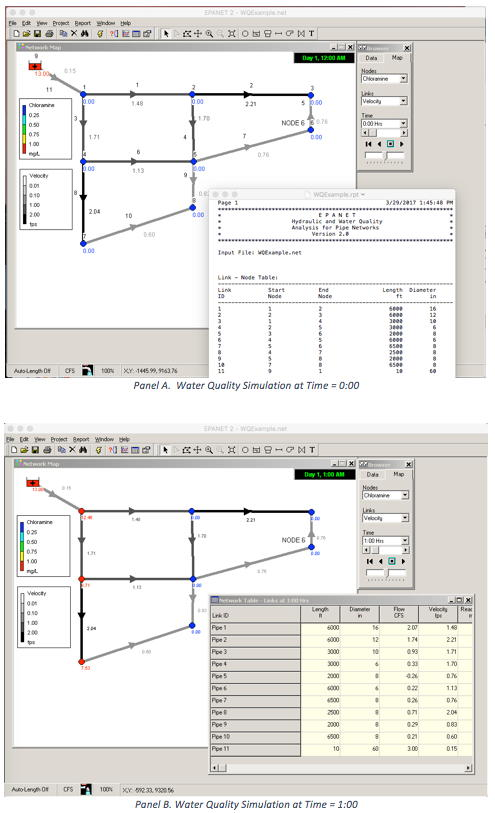
\includegraphics[width=4.5in]{WaterQuality-1.jpg}
     \caption{EPA-NET Water Quality Simulation; Hours 0:00 and 1:00}
   \label{fig:waterQ1} 
\end{figure}

\begin{figure}[ht!] %  figure placement: here, top, bottom, or page
\centering
   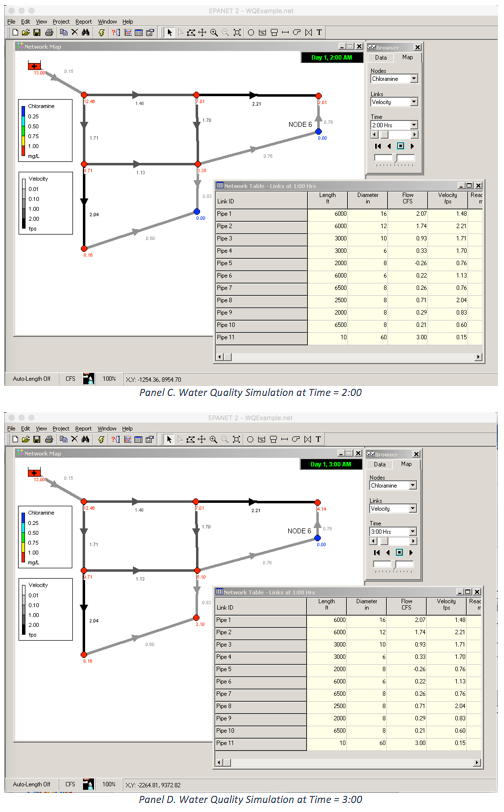
\includegraphics[width=4.5in]{WaterQuality-2.jpg}
     \caption{EPA-NET Water Quality Simulation; Hours 2:00 and 3:00}
   \label{fig:waterQ2} 
\end{figure}

\begin{figure}[ht!] %  figure placement: here, top, bottom, or page
\centering
   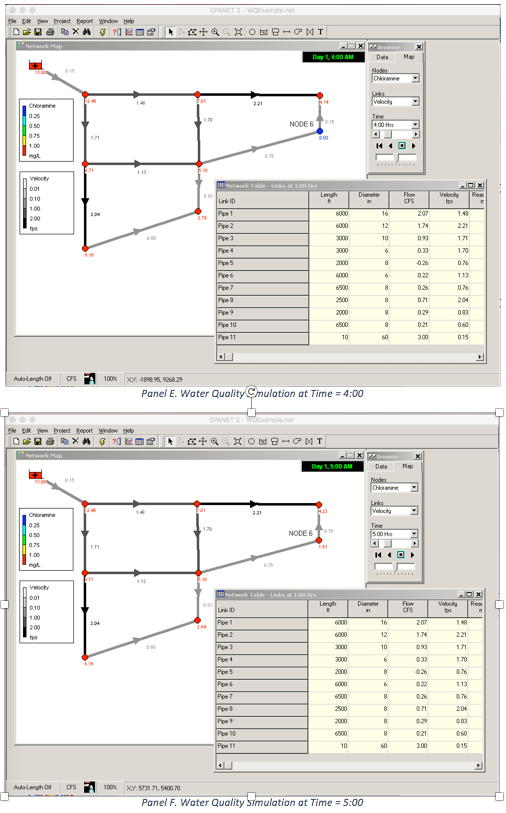
\includegraphics[width=4.5in]{WaterQuality-3.jpg}
     \caption{EPA-NET Water Quality Simulation; Hours 4:00 and 5:00}
   \label{fig:waterQ3} 
\end{figure}
\clearpage

\end{enumerate}

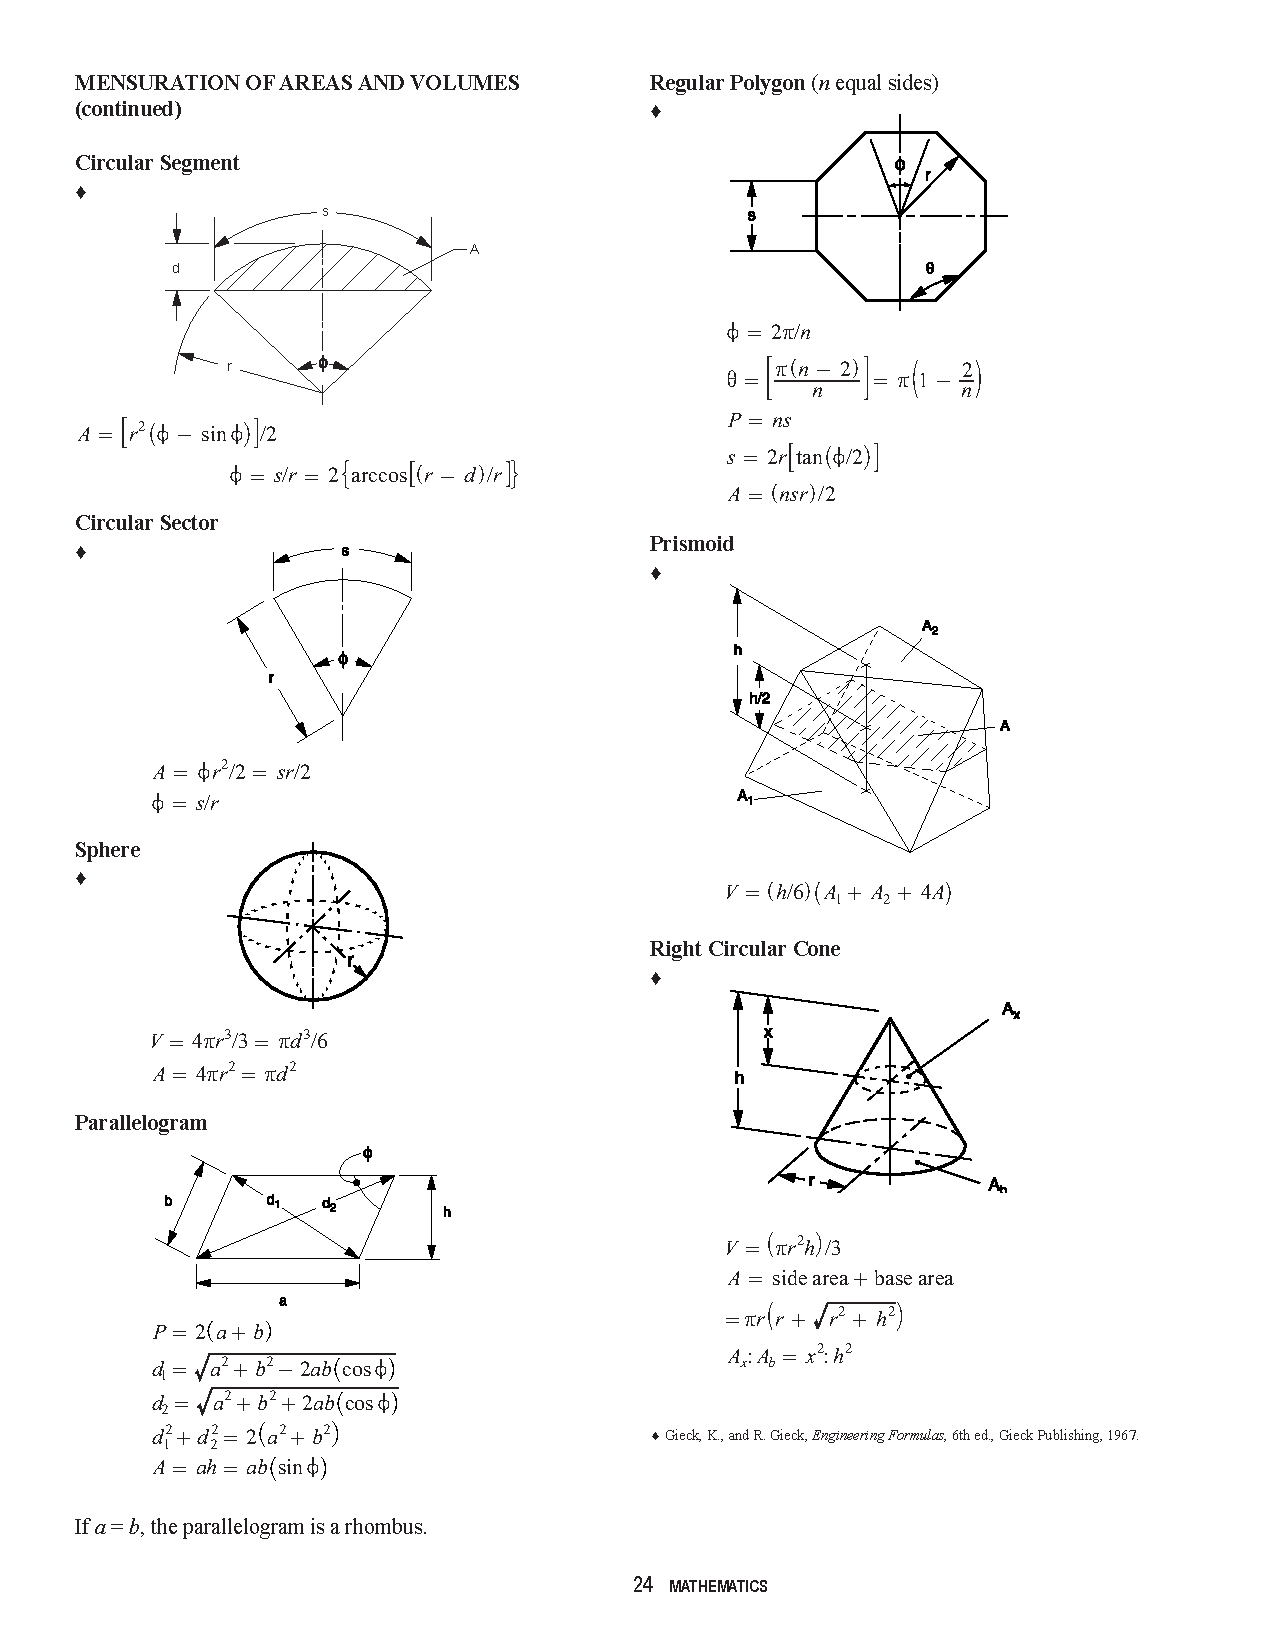
\includepdf[pages=1]{FER-p1.pdf}
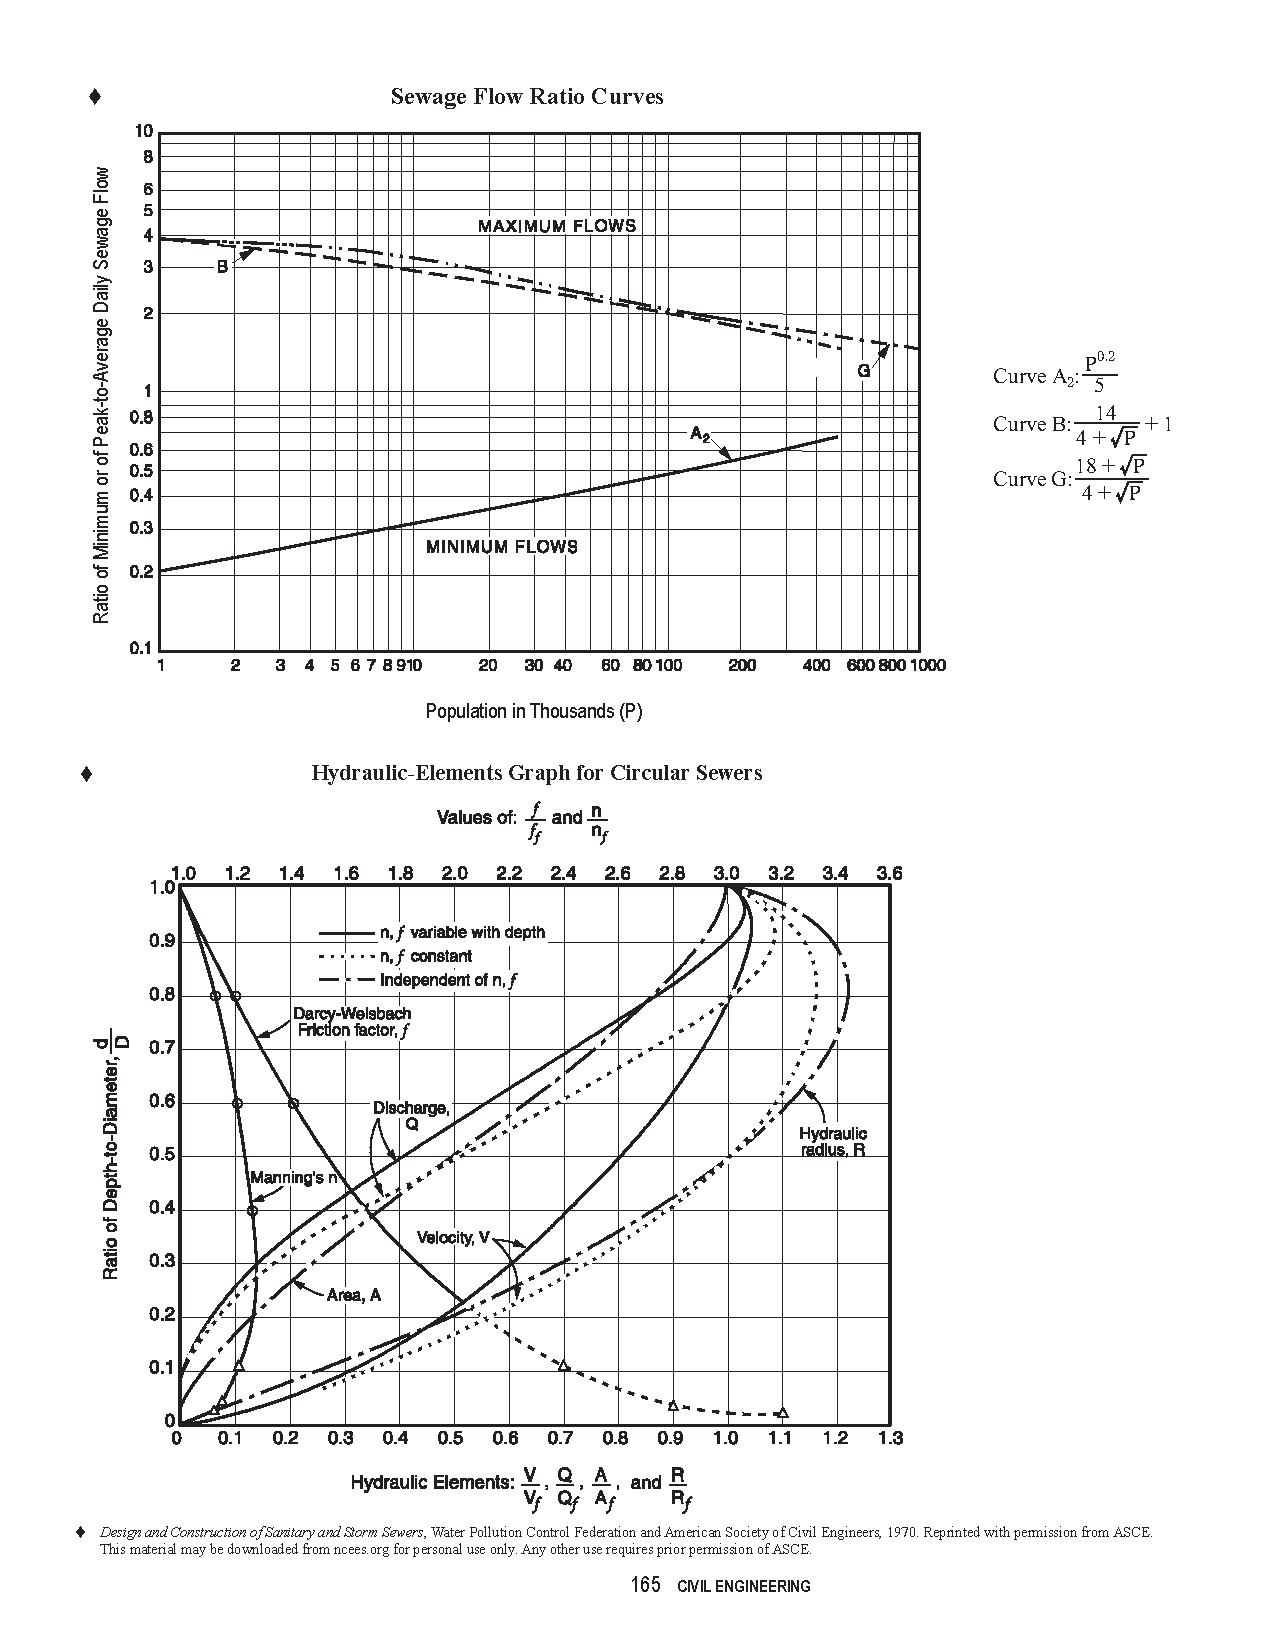
\includepdf[pages=1]{FER-p2.pdf}
\end{document}  




